\documentclass[crop,border=7pt]{standalone}
\usepackage{tikz}
\usepackage{ifthen}
\usetikzlibrary{shapes.geometric}
\begin{document}
  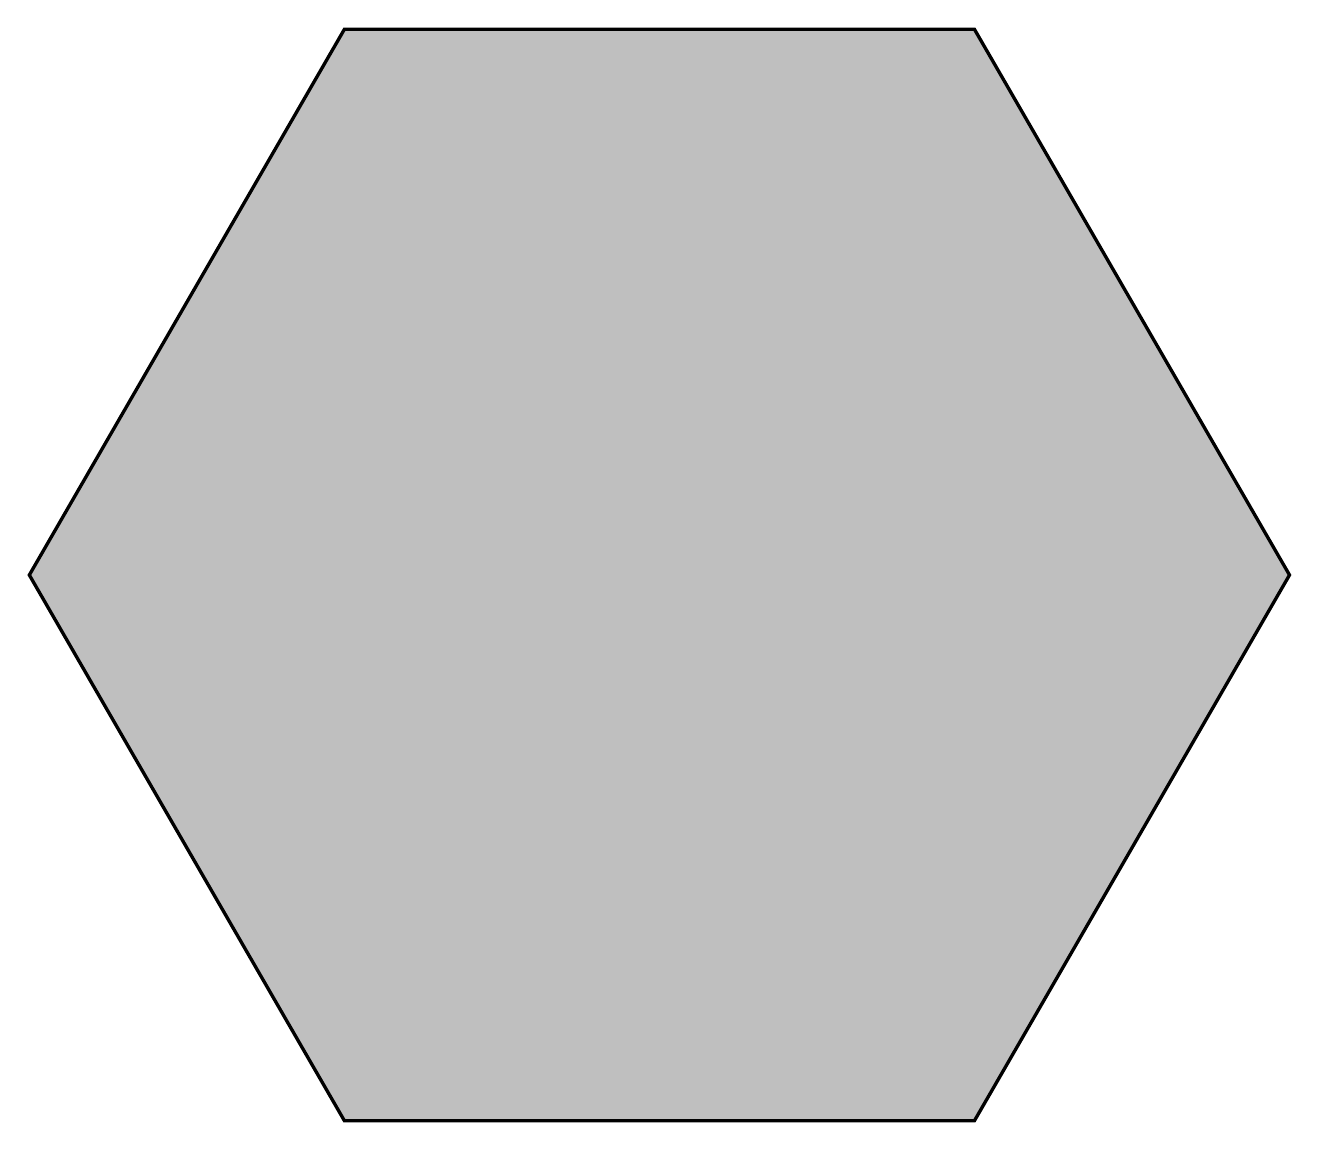
\begin{tikzpicture}[
  blacknode/.style={shape=circle, draw=black, line width=1, fill=gray },
  bluenode/.style={shape=circle, draw=black, line width=1, fill=blue },
  greennode/.style={shape=circle, draw=black, line width=1, fill=green },
  rednode/.style={shape=circle, draw=black, line width=1, fill=red },
  yellownode/.style={shape=circle, draw=black, line width=1, fill=yellow },
  violetnode/.style={shape=circle, draw=black, line width=1, fill=violet },   
  graynode/.style={shape=circle, draw=black, line width=1, fill=blue!10 },  
]
%%%hexagon
\newdimen\R
  \R=8.002074731cm
  \coordinate (center) at (0,0);
 \filldraw[gray!50, draw=black, very thick] (0:\R)
     \foreach \x in {60,120,...,360} {  -- (\x:\R) }
              -- cycle (300:\R)
              -- cycle (240:\R) 
              -- cycle (180:\R) 
              -- cycle (120:\R) 
              -- cycle (60:\R) 
              -- cycle (0:\R) ;
%%%%%%%%%

              
  \end{tikzpicture}
\end{document}